



	\begin{minipage}{0.5\linewidth}
		
		\section{Verformungen}

		\subsection{Verformung am Zugstab}
		
			
	\textbf{Gerissen: (N > N$_r$) }
	
	\begin{tabular}{lp{0.3\linewidth}}
		
		Dehnung (Grenzfall im Riss):		& $ \varepsilon^{II} =  \frac{N}{A_s \cdot n \cdot E_c} $ \\
		
		Verformung (obere Schranke):		& $ \Delta l = l_0 \varepsilon^{II} $ \\
		
		Mitwirkung zwischen den Rissen	& \\
		
		Kriechen:						& kein Einfluss, da keine Druckbeanspruchung im Beton \\
		
	\end{tabular}
	
\end{minipage}
\begin{minipage}{0.5\linewidth}
		
		
		\textbf{Ungerissen: (N < N$_r$) }
		
		\begin{tabular}{ll}
			Dehnung:		& $ \varepsilon = \frac{N}{A_i \cdot E_c} $ \\
			
			Verformung:		& $ \Delta l = l_0 \varepsilon $ \\
			
			Schwinden:		& Verformung \\
			
		\end{tabular}
				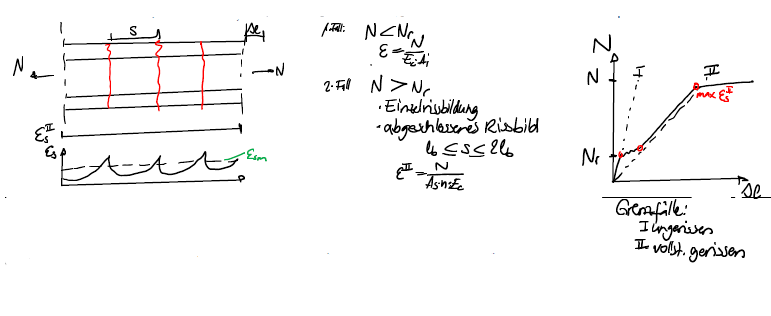
\includegraphics[width=\linewidth]{images/Verformung1Zustand.PNG}
	\end{minipage}


	\begin{minipage}{0.4\linewidth}
			\subsection{Berechnung von Verformung}
		
		SIA 262 4.4.3.2.4/5 (vereinfachte Durchbiegung), SIA 260 Anhang
		
		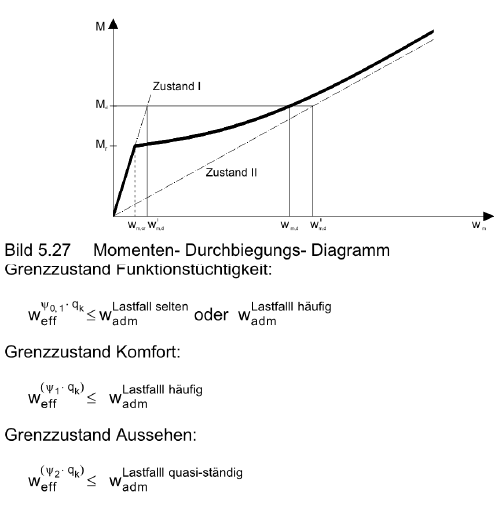
\includegraphics[width=\linewidth]{images/Verformung2Durchbiegung.PNG}
		
	\end{minipage}
	\begin{minipage}{0.5\linewidth}
		

		
		\begin{tabular}{p{0.35\linewidth}|p{0.4\linewidth}|p{0.3\linewidth}}
		
							
			Kriechen (Zustand 1) & $ EI^I = I^I \frac{E_{cm0}}{1 + \varphi} $	& $ \varphi \approx $ 2 (SIA 262) \\ \hline
			
			Schwinden(Zustand 1) &  & Verkürzung, Krümmung bei nicht-symmetrischem As \\
			Randspannungen	& $ \sigma_{co,u} = \frac{F}{A_{i \infty}} \mp \frac{F \cdot y_s}{I^I_{i \infty} } y_{o, u} $	& \\
			Schwindkrümmung	& $ \Delta \varepsilon_o = \frac{ \sigma_{co} }{E_{c \infty} }; \Delta \varepsilon_u = \frac{ \sigma_{cu} }{E_{c \infty} }; \kappa_s = \frac{|\Delta \varepsilon_o| + |\Delta \varepsilon_o|}{h} $ & Durchbiegung infolge Schwinden, kann häufig vernachlässigt werden \\ \hline

			
			Durchbiegung	& $ w = \int_{0}^{l} \frac{M}{EI} \bar{M} \cdot dx $	& $ \bar{M} $ = Moment aus virtuellem Belastungszustand \\
						&	& $ \frac{M}{EI} = \kappa $ = Durchbiegung \\ \hline
			
			Durchbiegung - vollständig gerissen & $ w_m = \frac{F \cdot l^3}{48EI_{II} } $	& extrem Fall, wenn i.O. $\rightarrow$ alles i.O. \\ \hline
			
			Durchbiegung - Bereich gerissen/ungerissen	& $ w_m = \frac{F \cdot l^3}{48EI_{II} } (1 - \zeta^3 (1 - \frac{EI_{II}}{EI_I} ) ) $ & \\
			
			
		\end{tabular}
		
		
	\end{minipage}